\chaptertitle{第五章\quad 组合方法}

排列关心的是"顺序"。但有大量问题只关心"选了哪些"，不关心"选出来之后怎么排"。组合就是研究这种"不计顺序"的选取方式。组合是排列的亲兄弟，但组合方法更丰富、更灵活——本章将学习组合、对应法、隔板法、算两次等核心工具。

\sectiontitle{5.1\quad 组合的定义}

先看两个问题：
\begin{enumerate}
\item 从$5$人中选$3$人排成一排领奖（分一、二、三等奖），有$A_5^3=60$种。
\item 从$5$人中选$3$人组成一个小组，不排名次，有多少种选法？
\end{enumerate}

问题$2$和问题$1$的区别在于：选出了$3$个人后，不用再考虑他们的内部顺序。也就是说，在问题$1$中，$(甲,乙,丙)$和$(乙,甲,丙)$算两种；在问题$2$中，$\{甲,乙,丙\}$就是同一个小组，不管内部顺序。

从$n$个不同元素中取出$m$个（$m\le n$），不计顺序，称为从$n$个中取$m$个的\textbf{组合}，记作$C_n^m$（有些书也记作$\binom{n}{m}$）。

组合数和排列数的关系：
\[
A_n^m = C_n^m \times A_m^m
\]
(先选$m$个出来，再给它们排顺序)$\quad\Rightarrow\quad
C_n^m = \frac{A_n^m}{A_m^m} = \frac{n!}{m!(n-m)!}
$

\begin{example}
从$8$人中选$3$人参加比赛，有多少种选法？
\end{example}
\begin{solution}
$C_8^3 = \dfrac{8\times7\times6}{3\times2\times1} = 56$种。
\end{solution}

几个具体例子，观察模式：
\[
C_5^2 = \frac{5\times4}{2}=10,\quad
C_5^3 = \frac{5\times4\times3}{3\times2\times1}=10,\quad
C_6^2 = \frac{6\times5}{2}=15
\]

\begin{example}
从$10$人中选$4$人参赛，有多少种选法？如果选$6$人不参赛呢？
\end{example}
\begin{solution}
选$4$人参赛：$C_{10}^4 = \dfrac{10\times9\times8\times7}{4\times3\times2\times1} = 210$种。\\
选$6$人不参赛：其实就是选$4$人参赛的另一种说法——$C_{10}^6 = C_{10}^4 = 210$种。
\end{solution}

\begin{exercise}
\item 计算：$C_7^3$，$C_8^2$，$C_{10}^3$。
\item 从$6$本书中选$2$本送人，有多少种送法？
\item 从$12$人中选$5$人组成篮球队，有多少种选法？
\end{exercise}

\sectiontitle{5.2\quad 组合恒等式}

组合数有两条非常重要的性质。我们不直接给出公式，而是先从具体例子中发现它们。

\begin{example}
计算$C_7^5$和$C_7^2$，$C_8^3$和$C_8^5$，你能发现什么规律？
\end{example}
\begin{solution}
$C_7^5 = 21$，$C_7^2 = 21$。$C_8^3 = 56$，$C_8^5 = 56$。\\
规律：$C_n^m = C_n^{n-m}$。\\
解释：从$n$个中选$m$个出来，等价于选$n-m$个留在原处。
\end{solution}

\begin{example}
计算$C_5^2 + C_5^3$和$C_6^3$，$C_4^2 + C_4^3$和$C_5^3$，你能发现什么规律？
\end{example}
\begin{solution}
$C_5^2 + C_5^3 = 10 + 10 = 20$，$C_6^3 = 20$。\\
$C_4^2 + C_4^3 = 6 + 4 = 10$，$C_5^3 = 10$。\\
规律：$C_n^m + C_n^{m+1} = C_{n+1}^{m+1}$（杨辉恒等式）。\\
解释：从$n+1$个中选$m+1$个，考虑某个特定元素——要么选它（再从剩下$n$个中选$m$个），要么不选它（再从剩下$n$个中选$m+1$个）。
\end{solution}

\textbf{组合恒等式}：
\begin{align}
C_n^m &= C_n^{n-m} \tag{对称性}\\
C_{n+1}^{m+1} &= C_n^m + C_n^{m+1} \tag{杨辉恒等式}
\end{align}

杨辉恒等式的几何意义就是杨辉三角中每个数等于它上方两数之和：
\begin{center}
\begin{tabular}{c|cccccc}
$n$ & & & & & & \\ \hline
$0$ & & & & $1$ & & \\
$1$ & & & $1$ & & $1$ & \\
$2$ & & $1$ & & $2$ & & $1$ \\
$3$ & $1$ & & $3$ & & $3$ & & $1$
\end{tabular}
\end{center}

\begin{exercise}
\item 利用$C_n^m = C_n^{n-m}$简化计算：$C_{100}^{98}$，$C_{50}^{48}$。
\item 验证杨辉恒等式：$C_6^2 + C_6^3 = C_7^3$。
\item 用组合意义解释$C_n^0 = 1$和$C_n^1 = n$。
\end{exercise}

\sectiontitle{5.3\quad 对应法（一一映射）}

对应法（也叫一一映射法）是组合数学中极为重要的思想：如果能在两个集合之间建立一个一一对应关系，那么它们的元素个数就相等。通过这个思路，我们可以把不熟悉的问题转化成熟悉的问题。

\begin{example}
一个集合$A=\{a,b,c\}$有多少个子集？利用对应法重新证明$2^n$规律。
\end{example}
\begin{solution}
每个元素要么选（$1$）要么不选（$0$）。一个子集对应一个长度为$3$的$0$-$1$串：
\[
\varnothing \leftrightarrow 000,\;
\{c\} \leftrightarrow 001,\;
\{b\} \leftrightarrow 010,\;
\{b,c\} \leftrightarrow 011,\;
\{a\} \leftrightarrow 100,\;
\{a,c\} \leftrightarrow 101,\;
\{a,b\} \leftrightarrow 110,\;
\{a,b,c\} \leftrightarrow 111
\]
$3$位$0$-$1$串有$2^3=8$种，所以$3$元集合有$8$个子集。一般地，$n$元集合有$2^n$个子集。
\end{solution}

\begin{example}
把$n$枚相同的硬币分给$k$个孩子（每个孩子可以分不到），有多少种分法？
\end{example}
\begin{solution}
设$n$枚硬币排成一行，在它们之间放$k-1$个隔板（包括两端外侧也可以放），每个孩子拿相邻两个隔板之间的硬币。
这等价于从$n+k-1$个位置（$n$枚硬币加$k-1$个隔板）中选$k-1$个放隔板：$C_{n+k-1}^{k-1}$种。\\
这就是下一节要学的隔板法，它的核心就是对应法——把"分硬币"对应成"选位置放隔板"。
\end{solution}

\begin{example}
从$n$个元素中选$m$个的组合$C_n^m$，能不能通过对应法用另一种方式表示？
\end{example}
\begin{solution}
每个组合对应一个$n$位$0$-$1$串，其中恰好有$m$个$1$（代表选中的$m$个元素）。比如$n=5,m=3$时，组合$\{2,4,5\}$对应$01011$。所以$C_n^m$就是$n$位$0$-$1$串中恰好有$m$个$1$的串的数量。
\end{solution}

\begin{exercise}
\item 有$4$盏灯排成一排，每盏可亮可灭。有多少种亮灭状态？用对应法解释。
\item $A=\{1,2,3,4,5\}$，一个子集对应一个$5$位二进制数。$01010$对应哪个子集？$\{1,3,5\}$对应哪个二进制数？
\end{exercise}

\sectiontitle{5.4\quad 标数法与隔板法}

\textbf{标数法}是用来计算最短路线数量的经典方法。

\begin{example}
在$3\times4$的网格中，从左上角$A$走到右下角$B$，每次只能向右或向下走一格。有多少条不同的最短路径？
\end{example}
\begin{solution}
最短路径需要向右走$4$步、向下走$3$步，共$7$步。\\
每一条路径对应一个顺序——在$7$个位置中选$3$个放"向下"（其余放"向右"）：$C_7^3 = 35$种。

也可以用标数法验证：在每个格子交点处标上到达该点的路线数。
\begin{center}
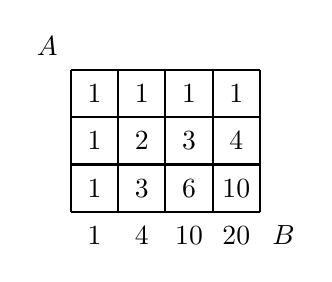
\begin{tikzpicture}[scale=0.6]
\draw[step=1,thick] (0,0) grid (4,3);
\node at (-0.5,3.5) {$A$};
\node at (4.5,-0.5) {$B$};
% 标数
\node at (0.5,2.5) {$1$};
\node at (1.5,2.5) {$1$};
\node at (2.5,2.5) {$1$};
\node at (3.5,2.5) {$1$};
\node at (0.5,1.5) {$1$};
\node at (1.5,1.5) {$2$};
\node at (2.5,1.5) {$3$};
\node at (3.5,1.5) {$4$};
\node at (0.5,0.5) {$1$};
\node at (1.5,0.5) {$3$};
\node at (2.5,0.5) {$6$};
\node at (3.5,0.5) {$10$};
\node at (0.5,-0.5) {$1$};
\node at (1.5,-0.5) {$4$};
\node at (2.5,-0.5) {$10$};
\node at (3.5,-0.5) {$20$};
\end{tikzpicture}
\end{center}
到达$B$（最右下角）为$20$——等一下，这里错了？

重新看：$3\times4$网格是说纵向$3$格、横向$4$格，即$4$条横线、$5$条竖线？不，需要统一理解方式。

通常标数法中，$m\times n$网格表示$m$行$n$列小方格，从左上角到右下角要走$m$步向下、$n$步向右，共$m+n$步，选$m$步向下：$C_{m+n}^m$种。\\
$3\times4$网格（$3$行$4$列小方格）：$C_7^3 = 35$种。
\end{solution}

\textbf{隔板法}——将标数法抽象化。

隔板法解决这样的问题：把$n$个相同的物品分给$k$个人（允许有人分不到），有多少种分法？

设想$n$个物品排成一行，在它们之间（包括两端）插入$k-1$个隔板，第$i$个人拿第$i-1$个和第$i$个隔板之间的物品。每个隔板的位置选法对应一种分配方案。

$n$个物品和$k-1$个隔板，共$n+k-1$个位置。选$k-1$个位置放隔板（或选$n$个位置放物品）：
\[
C_{n+k-1}^{k-1} = C_{n+k-1}^{n}
\]

\begin{example}
把$10$个相同的苹果分给$3$个小朋友（可以有人不分到），有多少种分法？
\end{example}
\begin{solution}
$n=10$，$k=3$：$C_{10+3-1}^{3-1} = C_{12}^2 = 66$种。
\end{solution}

变体：如果要求每人至少分到$1$个呢？

先给每人$1$个，剩下$n-k$个再随意分（允许有人再得$0$个）：
\[
C_{(n-k)+k-1}^{k-1} = C_{n-1}^{k-1}
\]

\begin{example}
把$10$个相同的苹果分给$3$个小朋友，每人至少$1$个，有多少种分法？
\end{example}
\begin{solution}
先每人给$1$个，剩下$7$个随意分：$C_{7+3-1}^{3-1} = C_9^2 = 36$种。

或者用公式：$C_{10-1}^{3-1} = C_9^2 = 36$种。
\end{solution}

\begin{example}
方程$x+y+z=10$有多少组非负整数解？有多少组正整数解？
\end{example}
\begin{solution}
非负整数解：把$10$个$1$分给$x,y,z$三个变量，允许为$0$。$C_{10+3-1}^{3-1}=C_{12}^2=66$组。\\
正整数解：先给每个变量$1$，剩下$7$个随意分。$C_{10-1}^{3-1}=C_9^2=36$组。
\end{solution}

\begin{exercise}
\item $2\times3$网格（$2$行$3$列）中从左上到右下的最短路径有多少条？
\item 把$8$本相同的笔记本分给$4$名学生，每人至少$1$本，有多少种分法？
\item 方程$a+b+c+d=15$有多少组正整数解？
\end{exercise}

\sectiontitle{5.5\quad 算两次（双重计数）}

"算两次"是一种极其巧妙的证明方法：用两种不同的方式计算同一个数量，得到的结果必然相等。由此可以推导出恒等式。

\begin{example}
从$n$个人中选一个$k$人委员会并指定其中一人当主席，有多少种方式？
\end{example}
\begin{solution}
算两次：\\
方法$1$：先选委员会（$C_n^k$种），再从委员会$k$人中选主席（$k$种）：$kC_n^k$。\\
方法$2$：先选主席（$n$种），再从剩下$n-1$人中选$k-1$个委员：$nC_{n-1}^{k-1}$。\\
两种方式结果相等：$kC_n^k = nC_{n-1}^{k-1}$，即$C_n^k = \dfrac{n}{k}C_{n-1}^{k-1}$。
\end{solution}

\begin{example}
利用算两次证明杨辉恒等式：$C_{n+1}^{m+1} = C_n^m + C_n^{m+1}$。
\end{example}
\begin{solution}
从$n+1$个元素中选$m+1$个。考虑某个特殊元素$a$：\\
要么$a$被选中——再从剩下$n$个中选$m$个：$C_n^m$种。\\
要么$a$不被选中——再从剩下$n$个中选$m+1$个：$C_n^{m+1}$种。\\
由加法原理：$C_{n+1}^{m+1} = C_n^m + C_n^{m+1}$。
\end{solution}

\begin{example}
证明：$C_n^0 + C_n^1 + C_n^2 + \cdots + C_n^n = 2^n$。
\end{example}
\begin{solution}
方法$1$（算两次）：$n$元集合的子集个数。\\
左边：按子集大小分类，大小为$k$的子集有$C_n^k$个，求和得到总子集数。\\
右边：每个元素选或不选，$2$种选择，共$2^n$种。\\
所以$\sum_{k=0}^n C_n^k = 2^n$。
\end{solution}

\begin{exercise}
\item 用算两次证明：$C_m^0C_n^k + C_m^1C_n^{k-1} + \cdots + C_m^kC_n^0 = C_{m+n}^k$（范德蒙恒等式）。（提示：从$m$男$n$女中选$k$人。）
\item 一个$n$边形有多少条对角线？用两种方法计算并相互验证。
\end{exercise}

\sectiontitle{5.6\quad 组合应用}

本节汇集排列组合的综合应用问题。

\textbf{握手问题}：$n$个人每两人握一次手，共握手多少次？
\[
C_n^2 = \frac{n(n-1)}{2}
\]

\begin{example}
$10$个人聚会，每两人握手一次，共握手多少次？
\end{example}
\begin{solution}
$C_{10}^2 = \dfrac{10\times9}{2} = 45$次。
\end{solution}

\textbf{分组分配问题}：把$n$个不同元素分成若干组，注意区分"分组"（组无标签）和"分配"（组有标签）。

\begin{example}
$6$人分成$3$组每组$2$人，有多少种分法？
\end{example}
\begin{solution}
先选第$1$组：$C_6^2$种。再选第$2$组：从剩下$4$人中选$2$人：$C_4^2$种。剩下$2$人是第$3$组：$C_2^2$种。
但$3$个组没有标签（比如$\{A,B\},\{C,D\},\{E,F\}$和$\{C,D\},\{A,B\},\{E,F\}$是同一种分法），所以要除以$3!$：
\[
\frac{C_6^2 \times C_4^2 \times C_2^2}{3!} = \frac{15\times6\times1}{6} = 15\ \text{种}
\]
\end{solution}

\textbf{混合问题}：同时用到排列和组合。

\begin{example}
从$5$名男生和$4$名女生中选$3$男$2$女排成一排，有多少种排法？
\end{example}
\begin{solution}
先选人：选$3$男$C_5^3$种，选$2$女$C_4^2$种，共$C_5^3\times C_4^2 = 10\times6 = 60$种选法。
再排列：$5$人全排列$5! = 120$种。\\
总数：$60\times120 = 7200$种。
\end{solution}

\begin{example}
$10$件产品中有$3$件次品。从中任取$4$件，求恰好有$2$件次品的取法。
\end{example}
\begin{solution}
从$3$件次品中选$2$件：$C_3^2=3$种。\\
从$7$件正品中选$2$件：$C_7^2=21$种。\\
总数：$3\times21 = 63$种。
\end{solution}

\begin{exercise}
\item $8$个球队单循环比赛（每两队赛一场），共需比赛多少场？
\item $5$本不同的书分给$3$个人，每人至少$1$本，有多少种分法？
\item 从$6$男$4$女中选$3$男$2$女组成一个$5$人小组，有多少种选法？
\end{exercise}

\sectiontitle{本章小结}

本章的核心是组合及其相关方法。组合$C_n^m$与排列$A_n^m$的关系是"先选后排"。组合恒等式（对称性、杨辉恒等式）是后续二项式定理的基础。对应法揭示了不同计数问题之间的内在联系。隔板法是解决"相同物品分配"问题的利器，其公式$C_{n+k-1}^{k-1}$对应标数法中的路径计数。算两次方法则给出了组合恒等式的优雅证明。

\sectiontitle{课后练习}

\subsection*{A组\quad 基础巩固}

\begin{exercise}
\item 计算：$C_9^3$，$C_{12}^4$，$C_8^5$。
\item 从$15$人中选$5$人参赛，有多少种选法？
\item 用隔板法：$12$个苹果分给$4$个小朋友，可以有人不分到，有多少种分法？
\item $2\times5$网格中从左上到右下的最短路径有多少条？
\item $10$个球队单循环，共比赛多少场？
\end{exercise}

\subsection*{B组\quad 挑战提升}

\begin{exercise}
\item 方程$x+y+z=20$有多少组正整数解？有多少组非负整数解？
\item 证明$C_n^0 + C_n^2 + C_n^4 + \cdots = 2^{n-1}$（奇数项组合数之和等于偶数项组合数之和）。（提示：用二项式定理，令$a=1,b=-1$。如果还没学，尝试用算两次。）
\item $8$本不同的书分给$3$个人，每人至少$2$本，有多少种分法？
\item 从$1$到$9$中选$3$个不同的数，使它们的和为偶数，有多少种选法？
\item 有$10$个相同的球和$4$个相同的盒子，每个盒子至少$1$个球，有多少种放法？
\end{exercise}

\vfill
\noindent\rule{\textwidth}{0.4pt}
本章练习答案请参见书末附录。
